\section{Publication and Data Relationships}
\label{sec:publication-data}
Figure~\ref{fig:data-detail} identifies the persistent relationships used by
publication and tutoring.
\begingroup
\setlength{\intextsep}{3pt}
\setlength{\abovecaptionskip}{4pt}
\begin{figure}[!ht]
\centering
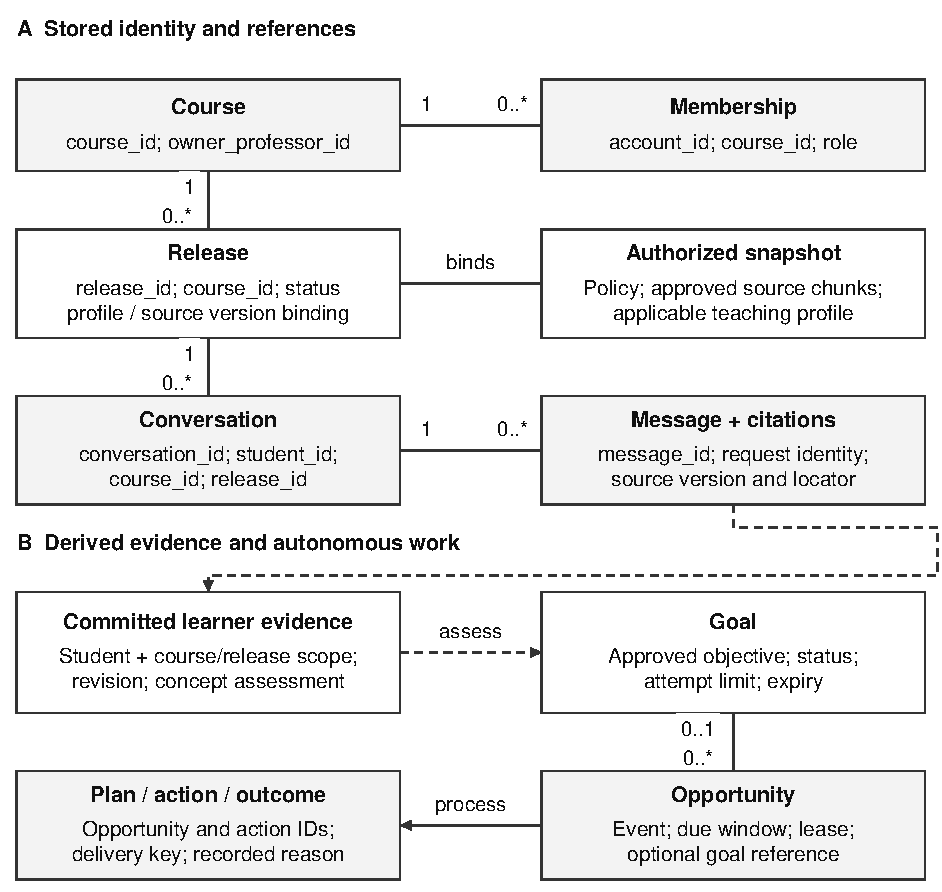
\includegraphics[width=\linewidth]{../../../reports/figures/course-twin-data-relationships.pdf}
\caption{Conceptual relationships among course releases, conversations, learner evidence and autonomous work.}
\label{fig:data-detail}
\end{figure}
\FloatBarrier
\endgroup
\clearpage
Publication is a separate state transition from preview or preflight.
Figure~\ref{fig:publication-detail} shows both operations and their failure
boundary. The preflight records deterministic readiness checks; it does not
replace the academic quality evaluations in the results section. The observer
runs after publication commits. Rollback revalidates and republishes a withdrawn release.
\begin{figure}[!ht]
\centering
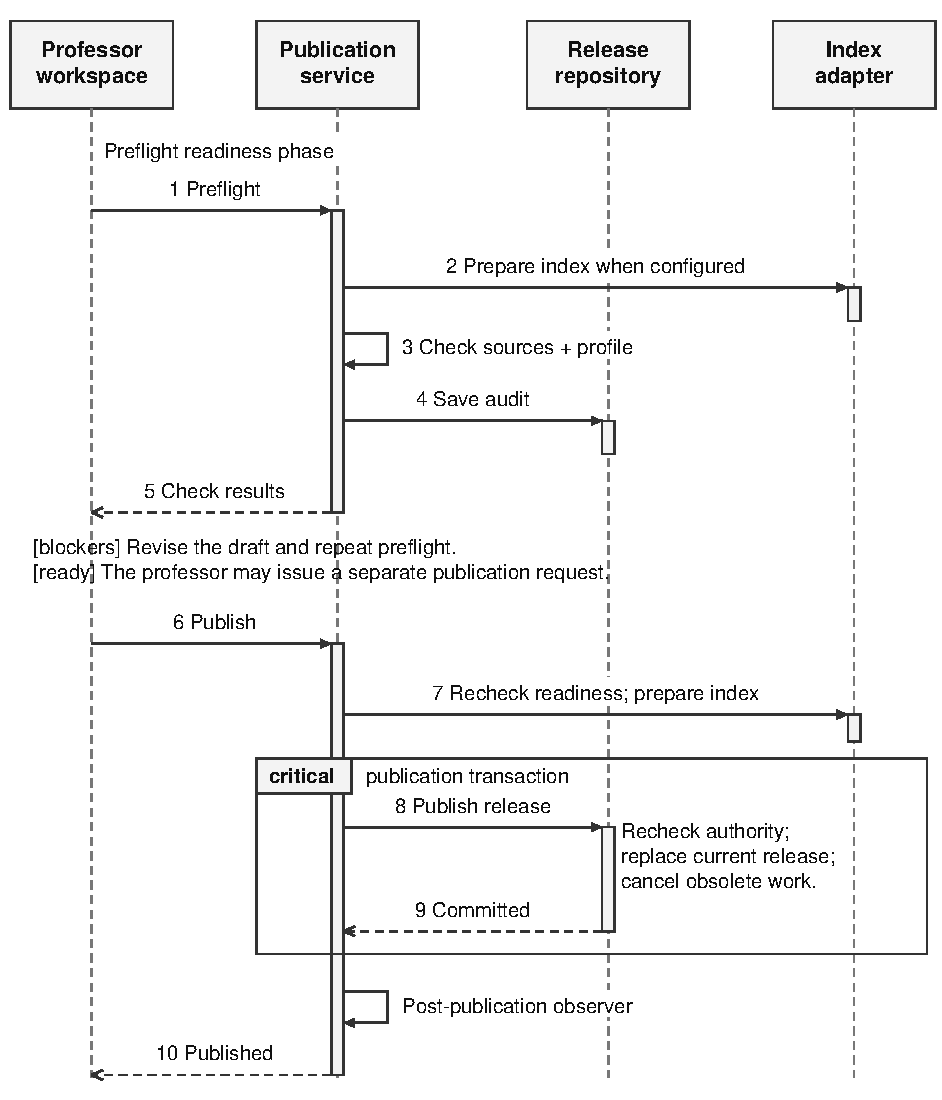
\includegraphics[width=\linewidth]{../../../reports/figures/course-twin-publication-sequence.pdf}
\caption{Preflight and publication interactions, with the release transaction shown explicitly.}
\label{fig:publication-detail}
\end{figure}
\FloatBarrier
